\documentclass{article}
\usepackage[utf8]{inputenc}
\usepackage{fullpage}
\usepackage{charter}
\usepackage{color}
\usepackage{graphicx}

\title{Background-aware Pose Recommendation for Daily Photography \textcolor{red}{(need to think later)}}
\author{Tian Li \\ (v-tili@microsoft.com, tian.li@pku.edu.cn) \\ Mentor: Steve Lin}
\date{January 2018}

\begin{document}

\maketitle

\section{Motivation}

%Describe the project here 

As of 2018, the picturing applications are ubiquitous. However, non-expert users may not take full advantage of these applications because they are not aware of any interesting poses fitting the specific background and they don't know any aesthetics rules that will guide them about where to stand. There is much recent work on pose or position recommendation, such as \cite{wang2015where2stand, xu2014should, ma2014pose, zhu2014mirror, fu2013data}. However, the previous work has several limitations. First, some of them only focuses on positions (i.e., where should the person stand) rather than poses. Second, they are not aware of the general background. \cite{fu2013data} considers only plane-like contexts and adopts heuristic rules to determine the context type. Third, they may have problems generalizing to various application scenarios. This is because some of the work models the problem as an image retrieval problem so the result will be affected by the incomplete image base a lot. Thus, 
we aim to develop an end-to-end learning-based model that takes as input an arbitrary background when taking pictures on mobile devices, and outputs one or several attractive poses as well as positions for the user.

\begin{figure}
    \centering
    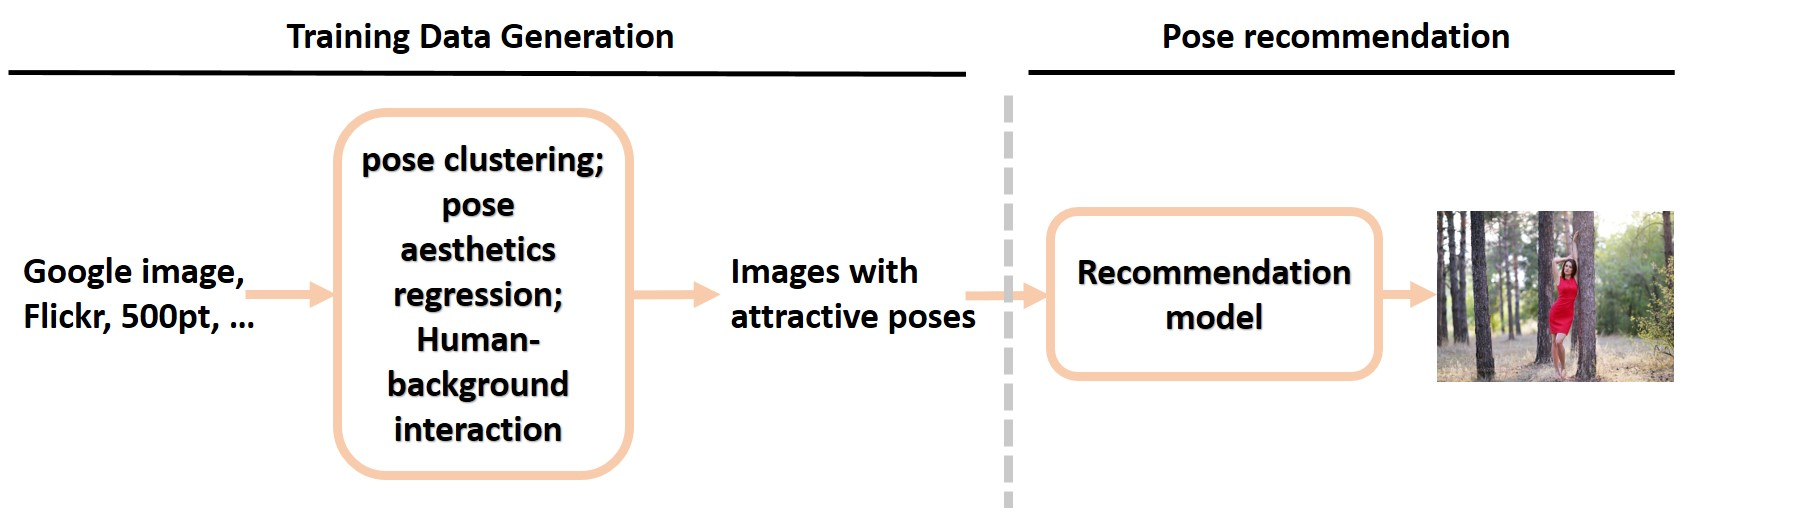
\includegraphics[scale=0.5]{figure/general}
    \caption{Caption}
    \label{fig:my_label}
\end{figure}

\section{Problem Definition}

\textbf{\emph{\underline{Goal}}} Our ultimate goal is formulated as follows:

\begin{itemize}
    \item Input: a background
 
    \item Output: the most interesting and attractive positions along with poses
\end{itemize}


Positions are easier to identify by leveraging common aesthetic rules such as rule of third \cite{}, xx and xxx. Therefore, we focus on recommending attractive poses for the user. First we need to obtain large amounts of professional training data. %How to generate them in an unsupervised way?

\subsection{\textbf{\emph{One core technical problem -- background-aware pose aesthetics evaluation}}}
We aim to generate large amounts of training data for pose recommendation in a(n) semi- or unsupervised way. Note that we can easily crawl or download thousands of images from the web. Then the problem comes to designing a background-aware pose aesthetic evaluation model to filter out those pleasing ones.

\noindent
\subsection{\textbf{\emph{The simplified problem -- human-background detection}}} 
From our observations, we find that directly assessing the aesthetic values of poses in terms of the scene may be too ambitious. With the assumption that all attractive poses are those having interaction with the background, we would like to detect if the person in the image have some kind of interactions with the environment and then consider the images involving interaction as samples with interesting poses. This is a classification problem with a human and a background object as input and a binary label as output.



\textbf{\emph{\underline{}}}

\section{Approaches}

\subsection{Image preprocessing}

We restrict the training data to contain only one person. So we run human detection on all raw images to drop those containing zero or multiple persons.

\subsection{Background-aware pose aesthetics evaluation}
    Our first attempt is to directly access the aesthetic values of the poses in a weakly-supervised fashion. The most attractive poses with respect to a scene will be included in the training set. More specific, we have tried the following two approaches:

    \begin{enumerate}
        \item \textbf{(clustering)} For each background, \textbf{cluster} the poses so that we only need to label a few representative poses from each cluster. It's reasonable to consider all images from the same cluster having the same aesthetic values. In this way, maybe we can generate a bunch of training data quickly given the satisfying clustering results. Also, we expect that the clustering result will reveal some information about how ordinary poses look like, which should be very common in images from the web. In Figure 
        \ref{cluster}, which is my best-effort version of clustering, the results are not good. The features of the poses are extracted from a pre-trained pose estimation model \cite{insafutdinov2017cvpr}.  
        \item \textbf{(transfer learning)} For a mix of various backgrounds, we only label a small number of images, each with a value between $0$ and $9$ indicating their attractiveness with respect to the scene. Because of the few samples we have, we adopt a linear model (e.g., \emph{Lasso}) rather than a neural network to map the input features to the aesthetics value. We consider three sets of features: pose features, scene features and image composition features. The pose features are the same as those used in clustering. The scene features are represented by a 151-dimensional binary vector $S$, which is the scene parsing result using \emph{PSPNet} \cite{zhao2017pspnet}. $S[i]$ indicates whether the pre-defined $i$-$th$ scene appears in the image. The image composition features are a 4-dimensional vector $C$, with each dimension indicating the \emph{Rule of Third} value, the \emph{Visual Balance} value, the \emph{Diagonal Dominance} value and the \emph{Object Size} value respectively \footnote{https://github.com/posgraph/coupe.composition-score-calculator}. After training a linear regressor on top of those features, we apply the model to large datasets. However, this does not work well because of too many features and too few labeled data.
    \end{enumerate}
 
\begin{figure}
        \centering
        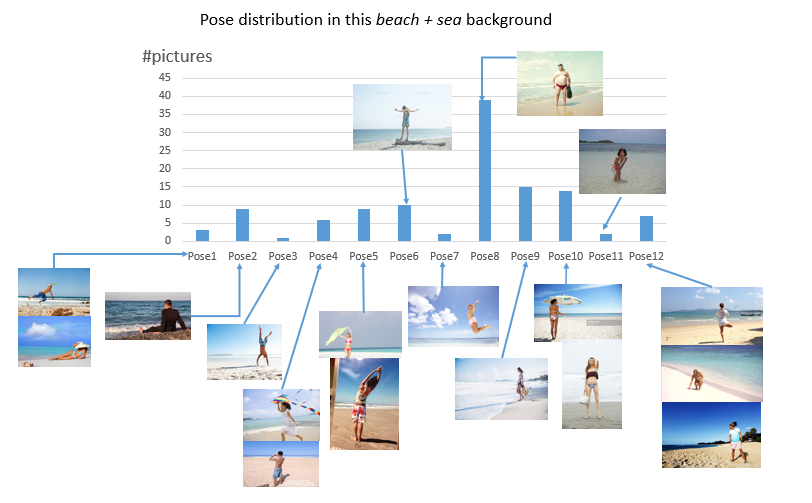
\includegraphics[scale=0.6]{figure/pose}
        \caption{Clustering result of the poses with the beach background}
        \label{cluster}
\end{figure}

\begin{figure}
        \centering
        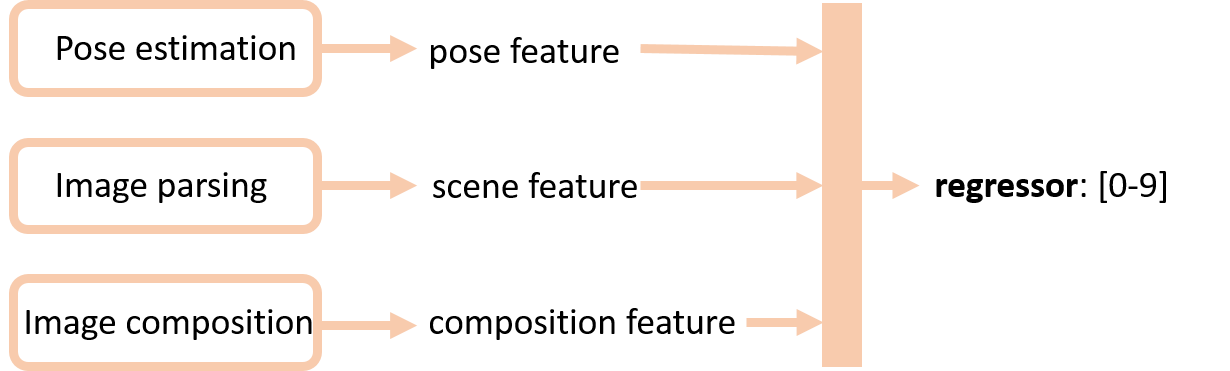
\includegraphics[scale=0.4]{figure/feature.png}
        \caption{Attempt of background-aware pose aesthetics assessment to generate training data}
        \label{cluster}
\end{figure}

\subsection{Human-background interaction detection}

Since defining the \emph{attractiveness} of poses seems to be too hard, we would like to mainly focus on human-background interactions. The assumption is that pictures with human-background interaction have large probabilities to contain pleasing poses. This is similar to some recent work in \emph{Human-Object Interaction (HOI)} detection \cite{chao:wacv2018}. But there are fundamental differences. 



\section{Challenges}

    \subsection{Lack of training data}
    
    \subsection{Modelling poses}
    
    \subsection{Modelling backgrounds}

\section{Future work}

\subsection{Some related work on modelling human object interaction (HOI)}

\bibliographystyle{acm}
\bibliography{reference}


\end{document}
